\section{Описание раздела <<Настройки>>}
\begin{enumerate}[\thesection .1]
\item Модуль служит для настройки параметров Системы.(рис.\ref {pic:pic17_1},\ref {pic:pic17_2}).\\
\begin{figure}[h!]
	\begin{floatrow}
		\ffigbox{\caption{Модуль настройки 1}\label{pic:pic17_1}}%
		{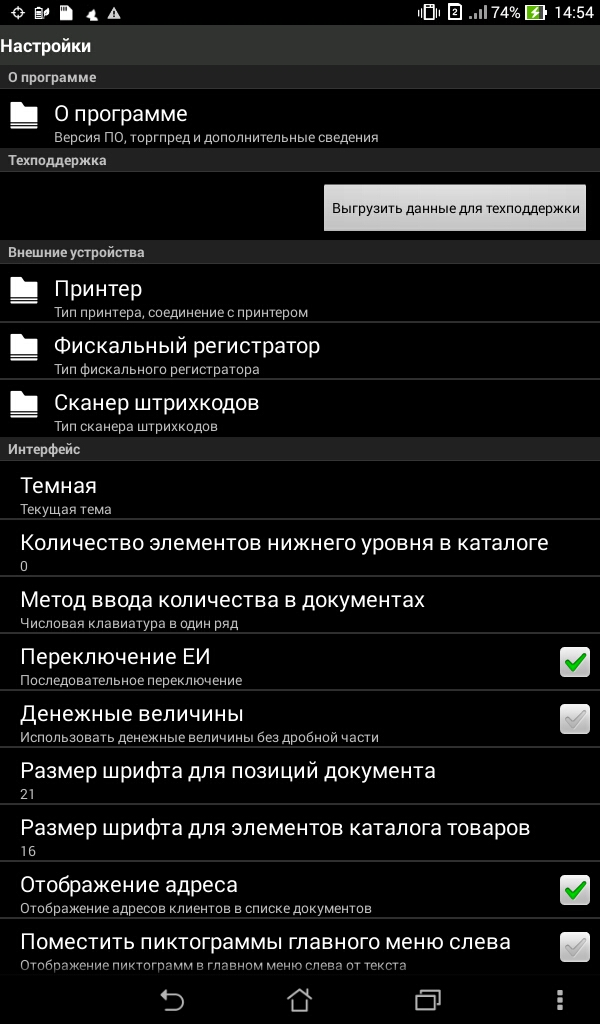
\includegraphics[width=0.6\linewidth]{scr17_1.jpg}}
		\ffigbox{\caption{Модуль настройки 2}\label{pic:pic17_2}}%
		{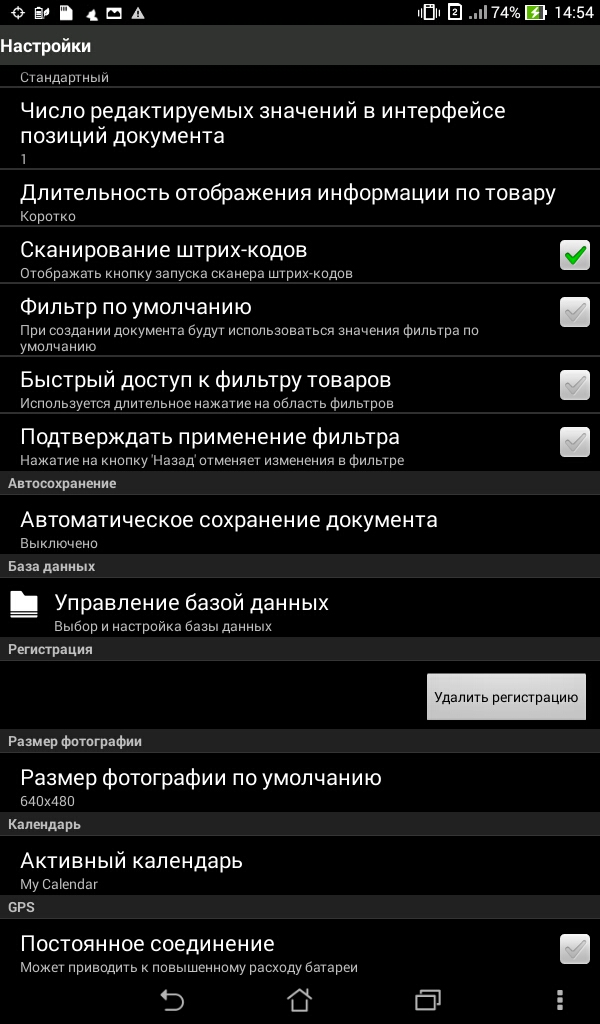
\includegraphics[width=0.6\linewidth]{scr17_2.jpg}}         
	\end{floatrow}
\end{figure}

\begin{longtable}{|p{5cm}|p{13cm}|}
\caption{Окно модуля содержит разделы, описанные в таблице ниже}\\
\hline	
\textbf{Название группы элементов} & \textbf{Описание группы элементов}\\ \hline
\endfirsthead
\hline
Название группы элементов & Описание группы элементов \\ \hline
\endhead
\hline
\multicolumn{2}{r}{Продолжение следует\ldots}\
\endfoot
\hline
\endlastfoot
%Название группы элементов & Описание группы элементов \\ \hline
О программе   & При касании на данном элементе открывается окно, где представлены следующие информационные поля: 
\begin{itemize}
	\item «Правовая информация»;
	\item «Версия Оптимум»;
	\item «Зарегистрировано» – содержит ФИО сотрудника, на которого произведена регистрация данного мобильного устройства в БД «Оптимум»;
\end{itemize} \\ \hline
Техподдержка  & Содержит кнопку, при нажатии на которую производится копирование служебных данных (логов, БД и настроек приложения) на SD-карту. Данные копируются в заархивированном виде.  \\ \hline
Внешние устройства  & Содержит поле «Принтер», по нажатию на которое открывается окно, в котором доступны следующие элементы:
 \begin{itemize}
 	\item «Тип принтера» - при касании на данном поле открывается окно выбора типа принтера (производителя);
 	\item «Тип соединения» - информационное поле, отображающее тип соединения с принтером;
 	\item «Имя (MAC-адрес) принтера» - при касании на данном поле открывается окно выбора принтера. В списке отображаются поддерживаемые Системой принтеры;
 \end{itemize} \\ \hline
Интерфейс  & Содержит поля:
\begin{itemize}
	\item «Количество элементов нижнего уровня в каталоге» - при касании на данном поле открывается окно для ввода значения данного параметра (N). Значение параметра определяет вид элемента иерархического списка - в каждом элементе списка будут показаны первые N значений из лежащего ниже уровня;
	\item «Вид клавиатуры» – параметр, который определяет, каким образом будет выглядеть клавиатура для ввода числовых значений (например, в окне ввода количества товарных позиций в документе). Возможны два режима: «Числовая клавиатура в один ряд» - цифры расположены в один ряд, «Увеличенная числовая клавиатура» - цифры расположены в два ряда;
	\item «Переключение ЕИ» - влияет на способ переключения единиц измерения товаров в документах. Возможны два режима:
	\begin{itemize}
		\item режим «Последовательное переключение»: при нажатии на кнопку единицы измерения (справа от поля ввода количества) происходит смена ЕИ для товарной позиции с ЕИ первого уровня на ЕИ второго уровня. Последующее нажатие приводит к смене ЕИ второго уровня на ЕИ третьего уровня и т. д;
		\item режим выбора: при нажатии на кнопку единицы измерения (справа от поля ввода количества) происходит открытие окна, где из списка выбирается необходимая ЕИ;
	\end{itemize}	
	\item «Денежные величины» (Использовать денежные величины без дробной части) - при активации данного режима все денежные величины (цены, суммы по документу) в приложении отображаются без дробной части. Дробная часть отсекается без округления;
	\item «Размер шрифта для позиций документа» - используется для установки размера шрифта при отображении информации о товарных позициях документа;
	\item «Размер шрифта для элементов каталога товаров» - используется для установки размера шрифта при отображении каталога товаров;
	\item «Отображение адреса» (Отображение адресов клиентов в списке документов) - при активации данного режима в списке созданных документов наряду с названием клиента отображается его адрес;
	\item «Компактный вид меню» (Использовать компактные строки в меню) - данный режим предназначен для отображения меню в более компактном виде (актуально, к примеру, для мобильных устройств с небольшим экраном);
\end{itemize}  \\ \hline
База данных  & Служебный функционал. Содержит поле «Управление базой данных», по нажатию на которое открывается окно просмотра доступных баз данных; \\ \hline
Регистрация  & Содержит кнопку «Удалить регистрацию», при нажатии на которую Система удаляет текущую регистрацию, после чего для работы с Системой необходима повторная регистрация и синхронизация устройства с сервером; \\ \hline
Размер фотографии  & Содержит поле «Размер фотографии по умолчанию», по нажатию на которое открывается окно выбора размера фотографий. Доступные размеры фотографий зависят от возможностей мобильного устройства; \\ \hline
Календарь  & Содержит поле «Активный календарь», по нажатию на которое открывается окно выбора календаря для отображения событий (задач), формируемых в модуле События;  \\ \hline
GPS  & Содержит поле «Приёмник GPS-координат», по нажатию на которое открывается окно выбора типа приёмника GPS-координат: \textbf{Location} или \textbf{NMEA}  \\ \hline
\end{longtable} 
\end{enumerate}